\fenicschapter{Finite Elements for Incompressible Fluids}
              {Finite Elements for Incompressible Fluids}
              {Andy R. Terrel, L. Ridgway Scott, Matthew G. Knepley, Robert C. Kirby and Garth N. Wells}
              {terrel}

The general structure of the finite element method (FEM) gives an overwhelming
number of choices for a simulation.  This is especially true for solving
incompressible fluids where theory points to many stable elements.  Finding the
best element for a particular code often depends on other criteria such as
coupling the solution to another simulation.  The modularity of the FEniCS
project allows users to quickly write simulations and choose a range of
elements that generate the simulation.  We leverage this modularity to
numerically study basic fluid modeling.

The \fenics{} project's automation tools provide a natural way to switch the
numerous elements of simulations, as studied in~\cite{TerrelScott2008}.  We
will use a steady state stokes equation and discuss a number of possible
elements, parameters, and solvers.  Additionally we give some numerical results
from a simple implementation.

\section{The Stokes Equation}
\label{terrel:section:Stokes}

The Stokes equation is the standard equilibrium equation for low Reynolds
number, incompressible flow.

  \begin{equation*}\label{terrel:eqn:StrongStokes}
    \begin{array}{c} -\Delta{\bf u} + \nabla{{\bf p}} = {\bf f} \\
     \nabla\cdot{{\bf u}} = 0\end{array}
 \end{equation*}

 The problem has been well studied and is documented in several
 books~\cite{BrennerScott2008, BrezziFortin1991}.  It is a challenging problem
 for a few reasons.  First, due to the coupling between the velocity and
 pressure results in a saddle point in the mixed variational form.  The matrix
 equations will be indefinite which proves to be quite taxing on iterative
 linear solvers. Second, the divergence free requirement on the velocity
 requires special care for the numerical discretization to preserve this
 property; it is often violated in common cases.

There are many stable methods for solving these equations but
 very few numerical studies including multiple methods. Often this is because
 it is so difficult to code one method that the cost outweighs the value of
 coding another method, especially if a large legacy simulation is already
 using one method.  With automated codes, meaningful comparisons are
 easily implemented; in the \fenics{} project, it is as simple as redefining the
 element or perhaps the variational form and new simulations are generated.

 Below is we provide a brief explanation of the different methods that were
 included in this study.  It is followed by a description of our testing
 framework and results from different methods.



\section{Numerical Formulations}

\subsection{Mixed method Formulation}

One of major challenges posed by the Stokes equation is handling the coupling
between the velocity and pressure.  One natural way to solve the system is to
create a mixed system, with blocks corresponding to fields, and each field
using a different element.  The variational form of this mixed system is as
follows:
\begin{quote}
  Let $V = H^1(\Omega)^n$ and $\Pi = \{q\in L^2(\Omega):\int_\Omega q
  dx = 0\}$. Given $F\in V'$, find functions ${\bf u}\in V$ and $p \in
  \Pi$ such that
\end{quote}
\begin{equation*}
\label{terrel:eqn:MixedStokes}
  \begin{array}{c}
    a({\bf u},{\bf v})+b({\bf v},p)  =  F({\bf v})\quad \forall v \in V\\
    b({\bf u},q) = 0\quad \forall q \in \Pi,
  \end{array}
\end{equation*}
where
\begin{eqnarray*}
  a({\bf u},{\bf v}) & := & \int_\Omega \nabla{{\bf u}}\cdot\nabla{{\bf v}} dx, \\
  b({\bf v}, q) & :=  & \int_\Omega (\nabla\cdot{{\bf v}}) q dx.
\end{eqnarray*}

This mixed method formulation uses two discrete spaces $V$ and $\Pi$.
Developing different finite element spaces for this system is quite challenging
due to Ladyzhenskaya-\babuska-Brezzi compatibility condition, see
Brezzi-Fortin for more details~\cite{Brezzi1974aFortin1991}.  Using the
most straight forward schemes such as continuous element spaces for both the
pressure and velocity leads to can to a over-determined system of equations.
Thus a range of scheme each varying in its ability to represent the solution
space accurately have been developed. This study presents some well known
elements and evaluates the numerical consequences of both.

\begin{figure}
  \centering
  \subfigure[$P_3$ for $V$]{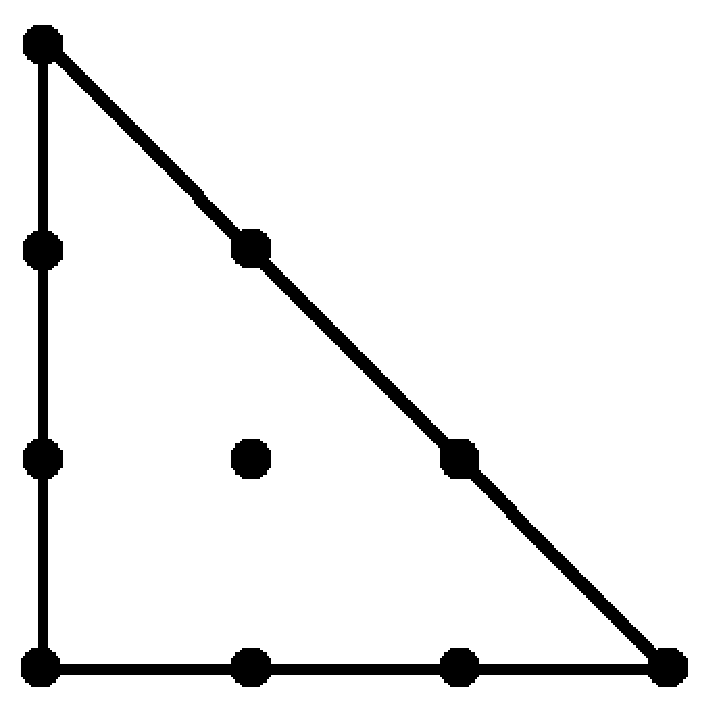
\includegraphics[scale=.3]{chapters/terrel/pdf/P3.pdf}}
  \hspace{2em}
  \subfigure[$P_2$ for $\Pi$]{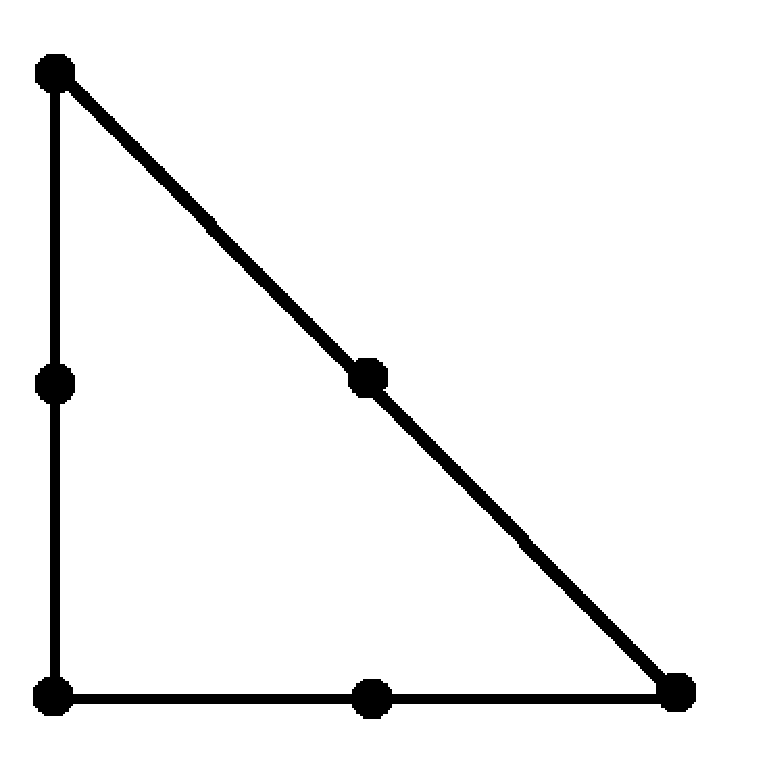
\includegraphics[scale=.3]{chapters/terrel/pdf/P2.pdf}}
  \caption{Taylor-Hood Elements}
  \label{terrel:fig:THElements}
\end{figure}

The Taylor-Hood element~\cite{Boffi1997,TaylorHood1973} is one of the most widely
used elements for solving Stokes flow.  It consists of a $P_k$ element for the
velocity space and $P_{k-1}$ for the pressure space (see
Figure~\ref{terrel:fig:THElements}).  Because of the simplicity of using Lagrangian
elements, it can easily be extended to higher orders. This element produces a
continuous pressure space, but the order of the pressure convergence is lower
than that for the velocity.

\begin{figure}
  \centering
  \subfigure[Crouzeix-Raviart for $V$]{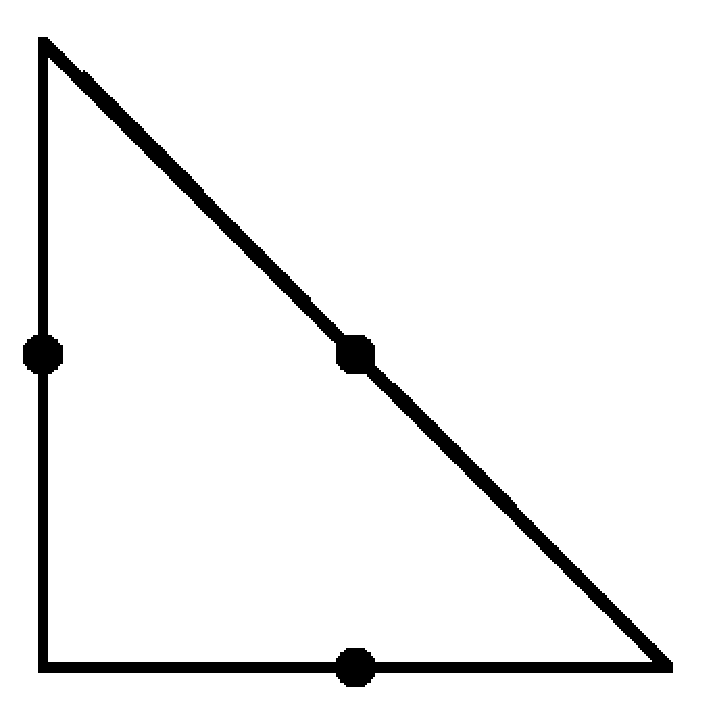
\includegraphics[scale=.3]{chapters/terrel/pdf/CR.pdf}}
  \hspace{2em}
  \subfigure[$P_0$ for $\Pi$]{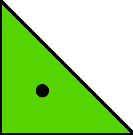
\includegraphics[scale=.3]{chapters/terrel/pdf/P0.pdf}}
  \caption{Crouzeix-Raviart Elements}
  \label{terrel:fig:CRElements}
\end{figure}

The Crouzeix-Raviart Element~\cite{CrouzeixRaviart1973} is a non-conforming element that uses
integral moments over the element edges as a basis for the velocity and a
discontinuous pressure space, $P_0$ (see Figure~\ref{terrel:fig:CRElements}).  For the
low order case, the velocity edge moments are equivalent to evaluating the
basis functions at the center of each edge.

Another possibility is just to use the high degree Lagrange element for
velocity but use a discontinuous element two orders lower in the pressure
space, what we loosely call CD.  Brezzi and Fortin discuss the $P_2-P_0$
case~\cite{Brezzi1974aFortin1991}, but for completeness we include higher order versions
as well.  For the low orders, the pressure is poorly approximated and the
element loses a degree of convergence.  This space does not satisfy the LBB
condition but is commonly used with a stabilization parameter or enriched with
bubble functions which are not discussed here.

\subsection{Stabilization}

To get around the difficulties of the LBB condition, there has been work on
stabilization of the discrete problem.  Stabilization attempts to convert the
discrete problem from a saddle point to a positive definite matrix, for a more
complete discussion see Donea and Huerta~\cite{DoneaHuerta2003}.  The most
successful method has been the streamline upwind/Petrov-Galerkin (SUPG) method
of Brookes and Hughes~\cite{BrooksHughes1982}.  For our test with the Stokes problem, use
only the pressure stabilization from SUPG changes the variational problem to the following:

\begin{equation*}
\label{terrel:eqn:StabilizedStokes}
\begin{array}{c}
  a({\bf u},{\bf v})+b({\bf v},p) + (\delta\cdot\nabla{q},\nabla{p})  =  ({\bf v},
  {\bf f}) + (\delta\cdot\nabla{q}, \bf f)\\
  b({\bf u},q) = 0
  \end{array}
\end{equation*}

where $\delta$ is a stabilization parameter, for our tests it was set to 0.2
times the circumference of the mesh cell squared.  The tests stabilize the
simple element that uses continuous elements of the same order for both the
pressure and velocity spaces, which we call STAB.  Additionally we apply the
stabilization parameter the Taylor-Hood element, TH\_STAB, and get a improved convergence
rate.

\subsection{Iterated Penalty Method}

Other solutions to avoid the LBB condition and the saddle point problem are the
Uzawa iteration method and penalty methods.  A combination of these two
ingredients results in the iterated penalty method or Scott and
Vogelius~\cite{ScottVogelius1985}. Let $r,\rho\in\R$ and $\rho > 0$ and define
${\bf u}^n$ and ${\bf w}^n$ by

\begin{align*}
\label{terrel:eqn:IPStokes}
 a({\bf u}^n,{\bf v})+r(\nabla\cdot{\bf u}^n,\nabla\cdot{v}) &=  F({\bf v}) - (\nabla\cdot{\bf v},\nabla\cdot{\bf w}^n)\\
  {\bf w}^{n+1} &= {\bf w}^n + \rho{\bf u}^n
\end{align*}


The pressure may be recovered from the auxiliary ${\bf w}$ field, $p = \nabla\cdot{\bf
  w} - C$ were $C$ is a constant, we use the average of $\nabla\cdot{\bf w}$ to center
around zero. The algorithm assumes ${\bf w^0} = \bf{0}$, solves the first
equation updating $\bf{w}$ every step it finds a fixed point, $||u^{n+1} -
u^{n}|| < \epsilon$. This method uses only one space, but requires a higher
order continuous element \cite{ScottVogelius1985a} and it solves the divergence free
criteria exactly.  The iteration count and accuracy is dependent upon
the penalty coefficients $\rho$ and $r$.  For our experiments we use ${\rho =
  -r = 1.0e3}$.

\section{Numerical Tests}
\label{terrel:sec:Results}

\begin{figure}[ht]
\centering
\subfigure[Unit square mesh 16x16 with cross pattern]{
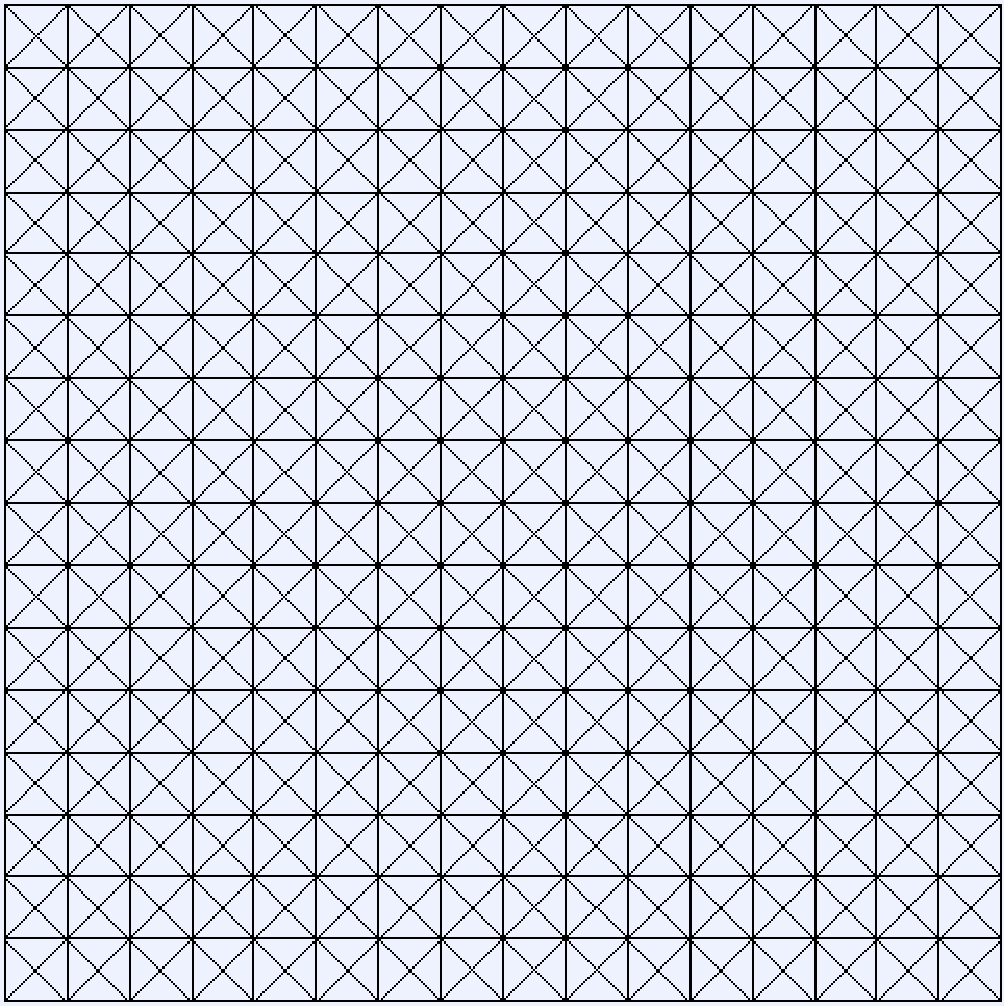
\includegraphics[scale=.25]{chapters/terrel/pdf/mesh.pdf}
\label{terrel:fig:mesh}
}
\qquad
\subfigure[Velocity magnitude of test problem]{
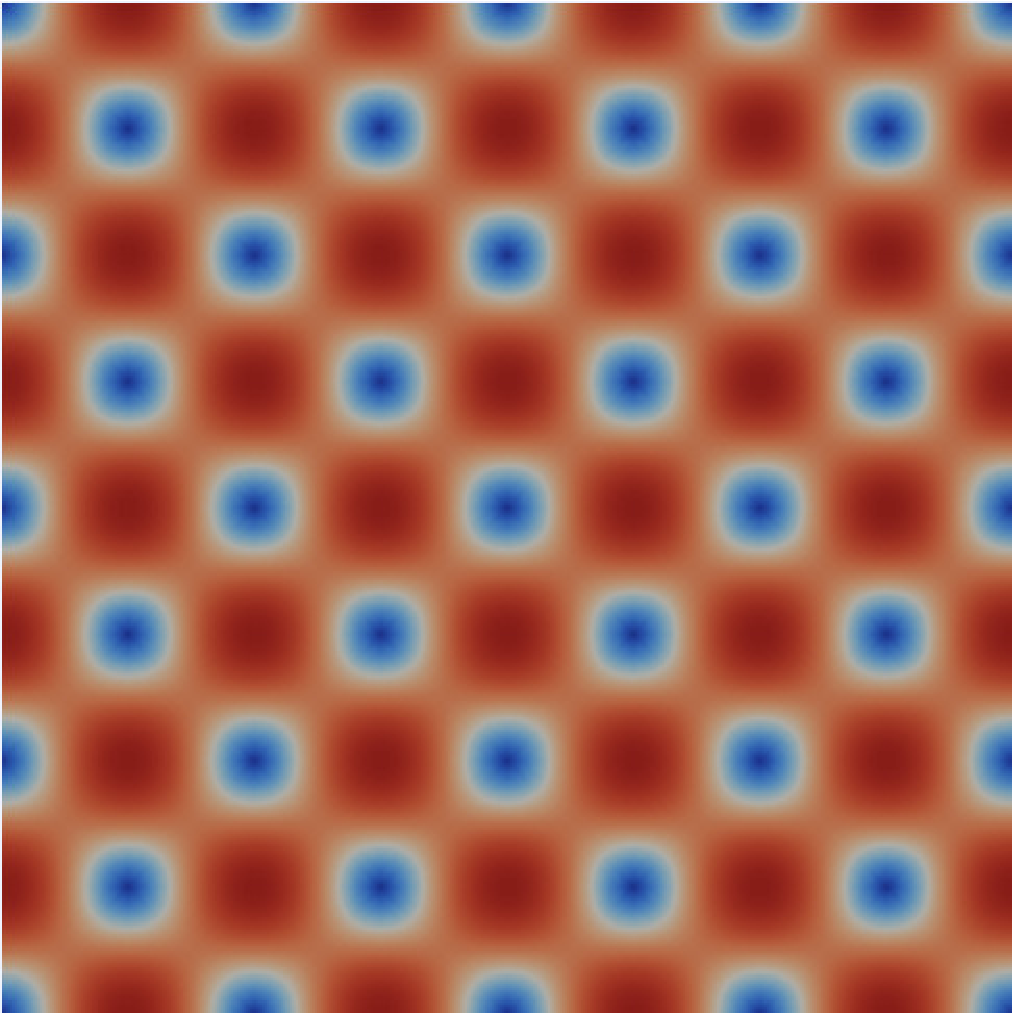
\includegraphics[scale=.25]{chapters/terrel/pdf/vel_test.pdf}
\label{terrel:fig:vel_test}
}
\qquad
\subfigure[Velocity magnitude of lid driven cavity with streamlines]{
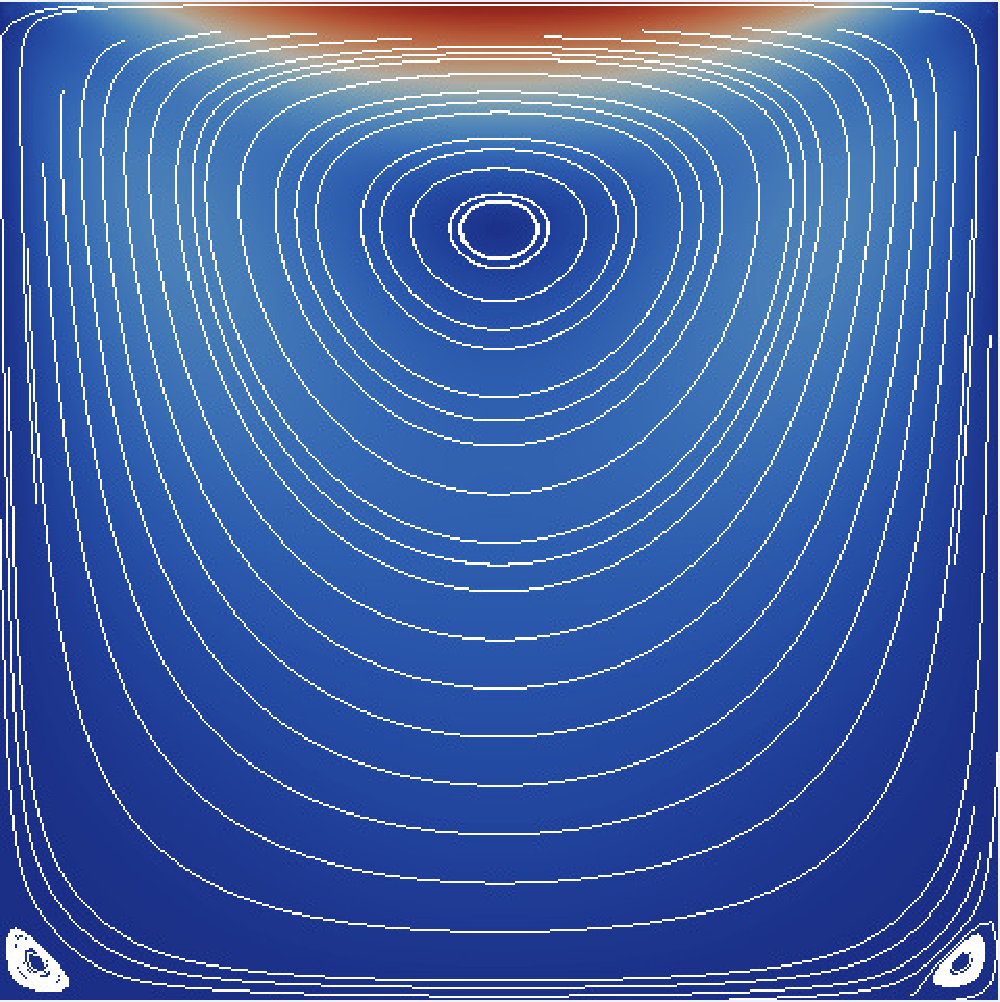
\includegraphics[scale=.25]{chapters/terrel/pdf/vel_lid.pdf}
\label{terrel:fig:vel_lid}
}
\label{terrel:fig:meshsolution}
\caption{Test mesh and solution plots}
\end{figure}

In order to evaluate these methods, we will compare mesh sizes and element
orders on a test problem with an analytic solution and also compare the lid
driven cavity solutions as well.  All of the simulations used the \fenics{}
project to generate the discrete problems (\ffc{} v0.7.0,\dolfin{} v0.9.4,
\ufl{} v0.4.0, \ufc{} v1.2.0) with {UMFPACK}'s LU solver (from the
{SuiteSparse} package v3.4).  Because we are using direct linear
algegra solver, the number of degrees of freedom is a good measure of the total
work the method, this is not true for iterative solvers for such studies we
recommend the book by Elman, Silvester and Wathen\cite{ElmanEtAl2005}.  The
number of the degrees of freedom as a function of mesh size and element is
shown in Table~\ref{terrel:tab:DOFs}.

\subsection{Simulation Setup}

For our tests, we use a $n\times n$ unit square mesh with a cross pattern, see
Figure~\ref{terrel:fig:meshsolution} and use the following analytic solution:
\begin{equation*}
\label{terrel:eqn:testcase}
\begin{array}{rcl}
  {\bf f} &=& \left[\begin{array}{c} 28\pi^2\sin(4\pi x)\cos(4\pi y) \\
      -36\pi^2\cos(4\pi x)\sin(4\pi y)
    \end{array}\right]\\
  {\bf u} &=& \left[\begin{array}{c} \sin(4\pi x)\cos(4\pi y) \\
      -\cos(4\pi x)\sin(4\pi y)
    \end{array}\right] \\
  p &=& \pi*\cos(4\pi x)\cos(4\pi y)
\end{array}
\end{equation*}

To aid the linear solver we additionally ``pinpoint'' one pressure degree of
freedom to zero.  Because the pressure term is only determined up to a
constant, this process sets that constant and insures the space is not
singular. See
Figures~\ref{terrel:code:domain:test}~and~\ref{terrel:code:domain:lid} for the
definition of this domain in the Python interface.  The extension form the test
problem to the lid driven cavity is only a change in the boundary conditions
functions and right hand side equation.


Given a domain, we can define the variational problem over it, see
Figure~\ref{terrel:code:var:mixed}.  For the mixed methods the code can take a
pair of names for the element family and orders.  Additionally we can specify
to add stabilization terms.  \dolfin{} will use \ffc{} and \fiat{} to generate the
correct elements and forms automatically, allowing for one function to test all
the methods.  See Table~\ref{terrel:tab:element_vars} for a reference to the
names of each pair.  The iterated penalty method use can be defined generally
over the various orders but because the function space and solver is
significantly different we show the code in Figure~\ref{terrel:code:var:ip}.

To determine the error for the analytic problems, we compile a higher order
function space and project the solutions to that space.  Then we are able to
integrate over the domain, see Figure~\ref{terrel:code:error}.


\begin{figure}
\small
\begin{python}
# Define the boundary domains
class NoSlipDomain(SubDomain):
    def inside(self, x, on_boundary):
        return on_boundary

class PinPoint(SubDomain):
    def inside(self, x, on_boundary):
        return x[0] < DOLFIN_EPS and x[1] < DOLFIN_EPS

# Define mesh
mesh = UnitSquare(h_num, h_num, "crossed")

# Test problem specification
prob = {'f' : ("28*pi*pi*sin(4*pi*x[0])*cos(4*pi*x[1])",
                       "-36*pi*pi*cos(4*pi*x[0])*sin(4*pi*x[1])"),
            'u' : ("sin(4*pi*x[0])*cos(4*pi*x[1])",
                   "-cos(4*pi*x[0])*sin(4*pi*x[1])"),
            'p' : "pi*cos(4*pi*x[0])*cos(4*pi*x[1])"
    }

# Instantiate the boundary conditions
noslip_domain = NoSlipDomain()
noslip = Expression(prob['u'], V=V)
pinpoint = PinPoint()
pin_val = Expression(prob['p'], V=Q)
bc0 = DirichletBC(W.sub(0), noslip, noslip_domain)
bc1 = DirichletBC(W.sub(1), pin_val, pinpoint, "pointwise")
bc = [bc0, bc1]

# Define the RHS
f = Expression(prob['f'], V=V)

\end{python}
\label{terrel:code:domain:test}
\caption{Code for defining the test domain}
\end{figure}

\begin{figure}
\small
\begin{python}
# Define the boundary domains
class NoSlipDomain(SubDomain):
    def inside(self, x, on_boundary):
        return on_boundary and x[1] < 1.0 - DOLFIN_EPS

class Top(SubDomain):
    def inside(self, x, on_boundary):
        return on_boundary and x[1] > 1.0 - DOLFIN_EPS

class PinPoint(SubDomain):
    def inside(self, x, on_boundary):
        return x[0] < DOLFIN_EPS and x[1] < DOLFIN_EPS

# Define mesh
mesh = UnitSquare(h_num, h_num, "crossed")

# Instantiate the boundary conditions
noslip_domain = NoSlipDomain()
noslip_val = Constant(mesh, (0.0, 0.0))
top_domain = Top()
top_val = Expression(("x[0]*(1.0 - x[0])", "0.0"), V = V)
pinpoint = PinPoint()
pin_val = Constant(mesh, 0.0)

# Define the RHS
f = Constant(mesh, (0.0, 0.0))
\end{python}
\label{terrel:code:domain:lid}
\caption{Code for defining the lid domain}
\end{figure}


\begin{figure}
\small
\begin{python}
# Define function spaces
V = VectorFunctionSpace(mesh, V_element, V_order)
Q = FunctionSpace(mesh, P_element, P_order)
W = V + Q

# Define test and trial functions
(v, q) = TestFunctions(W)
(u, p) = TrialFunctions(W)

# Define the variational problems
a = (inner(grad(v), grad(u)) - div(v)*p + q*div(u))*dx
L = inner(v, f)*dx
if stabilized:
    h = CellSize(mesh)
    beta = 0.2
    delta = beta*h*h
    a += delta*inner(grad(q), grad(p))*dx
    L += inner(delta*grad(q), f)*dx
pde = VariationalProblem(a, L, bc)

# Assemble and solve
U = pde.solve()
\end{python}
\label{terrel:code:var:mixed}
\caption{Code for defining the various mixed methods, see
  Table~\ref{terrel:tab:element_vars}}
\end{figure}

\begin{table}
\centering
\caption{Element variables defining the different mixed methods}
\label{terrel:tab:element_vars}
\medskip
\small
\begin{tabular}{|cccccc|}
\hline
& Crouzeix-Raviart &  CD &  Taylor-Hood & STAB & TH\_STAB\\
\hline
{\tt V\_element } & {\tt "Crouzeix-Raviart"} &  {\tt "CG"} & {\tt
  "CG"} & {\tt "CG"} & {\tt "CG"}\\
{\tt V\_order} & $1$ & $p$ & $p$ & $p$ & $p$ \\
{\tt P\_element } & {\tt "DG"} &  {\tt "DG"} & {\tt "CG"} & {\tt "CG"} & {\tt "CG"}\\
{\tt P\_order} & $0$ & $p-2$ & $p-1$ & $p$ & $p-1$ \\
{\tt stabilized } & {\tt False} & {\tt False} &  {\tt False} & {\tt True} & {\tt True} \\
\hline
\end{tabular}
\end{table}


\begin{figure}
\small
\begin{python}
# Define function space
V = VectorFunctionSpace(mesh, "CG", V_order)

# Define test and trial functions
v = TestFunction(V)
u = TrialFunction(V)

# Define auxilary function and parameters
w = Function(V);  r = 1e3

# Define the variational problem
a = (inner(grad(v), grad(u)) - r*div(v)*div(u))*dx
L = (inner(v, f) + inner(div(v), div(w)))*dx
pde = VariationalProblem(a, L, bc0)

# Iterate to fix point
iters = 0; max_iters = 100; U_m_u = 1
while iters < max_iters and U_m_u > 1e-8:
    U = pde.solve()
    w.vector().axpy(c, U.vector())
    if iters != 0:
        U_m_u = (U.vector() - u_old_vec).norm('l2')
    u_old_vec = U.vector().copy()
    iters += 1
\end{python}
\label{terrel:code:var:ip}
\caption{Code for defining the iterated penalty methods}
\end{figure}

\begin{figure}
\small
\begin{python}
VP10 = VectorFunctionSpace(mesh, "CG", 10)
P10 = FunctionSpace(mesh, "CG", 10)
(u, p) = U.split(True)
u_ex = Expression(prob['u'], V=VP10)
M = inner((u_ex - u),(u_ex - u))*dx
v_err = assemble(M, mesh=mesh)
p_ex = Expression(prob['p'], V=P10)
Mp = (p_ex - p)*(p_ex - p)*dx
p_err = assemble(Mp, mesh=mesh)
Mdiv = div(u)*div(u)*dx
v_div = assemble(Mdiv, mesh=mesh)
\end{python}
\label{terrel:code:error}
\caption{Code for determining error of analytic problem.}
\end{figure}


\subsection{Results}


\begin{table}
  \centering
  \caption{A comparison of the degrees of freedom for each element organized by
    velocity order (p) and number of mesh divisions per dimension (m). A '-'
    indicate that the order for that particular element is not stable or undefined.}
  \label{terrel:tab:DOFs}
  \medskip
  \small
  \begin{tabular}{|cc|rrrrr|}
    \hline
    p & n & CR &  STAB & CD & TH & IP \\
    \hline
    1&  8 &   1056 &   435 & - & - & -  \\
      & 16 &   4160 & 1635 & - & - & - \\
      & 32 & 16512 & 6339 & - & - & - \\
    \hline
    2 &  8 & - &     1635 &  1346 &   1235 & - \\
       & 16 & - &    6339 &  5250 &   4771 & - \\
       & 32 & - &  24963 & 20738& 18755 & - \\
    \hline
    3 &  8 & - &    3603 &   3170 &   2947 & - \\
       & 16 & - & 14115 & 12482 & 11523 & - \\
       & 32 & - & 55875 & 49538 & 45571 & - \\
    \hline
    4 &  8 & - &    6339 &   5762 &    5427 &   4226 \\
       & 16 & - & 24963 & 22786 &  21347 & 16642 \\
       & 32 & - & 99075 & 90626 &  84675 & 66050 \\
    \hline
    5 &  8 & - &      9843 &     5762 &     8675 &     6562 \\
       & 16 & - &   38883 &   36162 &   34243 &   25922 \\
       & 32 & - & 154563 & 144002 & 136067 & 103042 \\
    \hline
\end{tabular}
\end{table}


In evaluating the method performance, a few features were
notable. Table~\ref{terrel:tab:vel_error} displays the calculated order of
convergence for each method and order, as calculated from a series of refined
meshes with $n$ in $\{8, 16, 32, 64\}$.  The optimal error should be $p + 1$
in the $L^2$ norm, notice the CD element loses one order of convergence due to
poor pressure estimation.  The difference in mass balance between the divergence free
elements and the continuous elements is clearly demonstrated in
Figure~\ref{terrel:fig:4th_Order_2:div}.  Runtimes for the mixed elements
parallel the number of degrees of freedom; however, the iterated penalty method
has better properties for iterative solvers making its increased runtime for
the small problems tested less important.  All runtimes were computed on a 2.6
GHz Intel Xeon with the timing the assembly and solve in the Python code,
assuming all code generation to be compile time.

\renewcommand\arraystretch{1.5}% (MyValue=1.0 is for standard spacing)
\begin{table}
  \centering
  \caption{Convergence rates of the velocity $L^2$ error for the different
    elements}
  \label{terrel:tab:vel_error}
  \small
  \begin{tabular}{|c|cccccc|}
    \hline
    p  & CR &  STAB &  CD  &TH & TH\_STAB &  IP \\
\hline
   1 & $2.01\pm1${\tt E}-$2$ & $1.93\pm6${\tt E}-$2$ & - & - & -  & -\\
   2 & -                 & $3.02\pm2${\tt E}-$2$ & $2.15\pm1${\tt E}-$1$ & $3.02\pm2${\tt E}-$2$ & $3.06\pm2${\tt E}-$2$ & -  \\
   3 & -                 & $4.00\pm1${\tt E}-$2$ & $3.11\pm2${\tt E}-$2$ & $3.98\pm1${\tt E}-$2$ & $4.00\pm4${\tt E}-$4$ & -  \\
   4 & -                 & $4.99\pm4${\tt E}-$3$ & $4.07\pm1${\tt E}-$2$ & $4.99\pm1${\tt E}-$3$ & $4.99\pm2${\tt E}-$3$ & $5.00\pm2${\tt E}-$3$\\
   5 & -                 & $5.98\pm1${\tt E}-$2$ & $5.1\pm5${\tt E}-$2$ & $5.97\pm1${\tt E}-$1$ & $5.97\pm1${\tt E}-$2$ & $5.97\pm1${\tt E}-$1$\\
    \hline
   \end{tabular}
\end{table}
\renewcommand\arraystretch{1}% (MyValue=1.0 is for standard spacing)


\begin{figure}
  \centering
  \subfigure[]{
    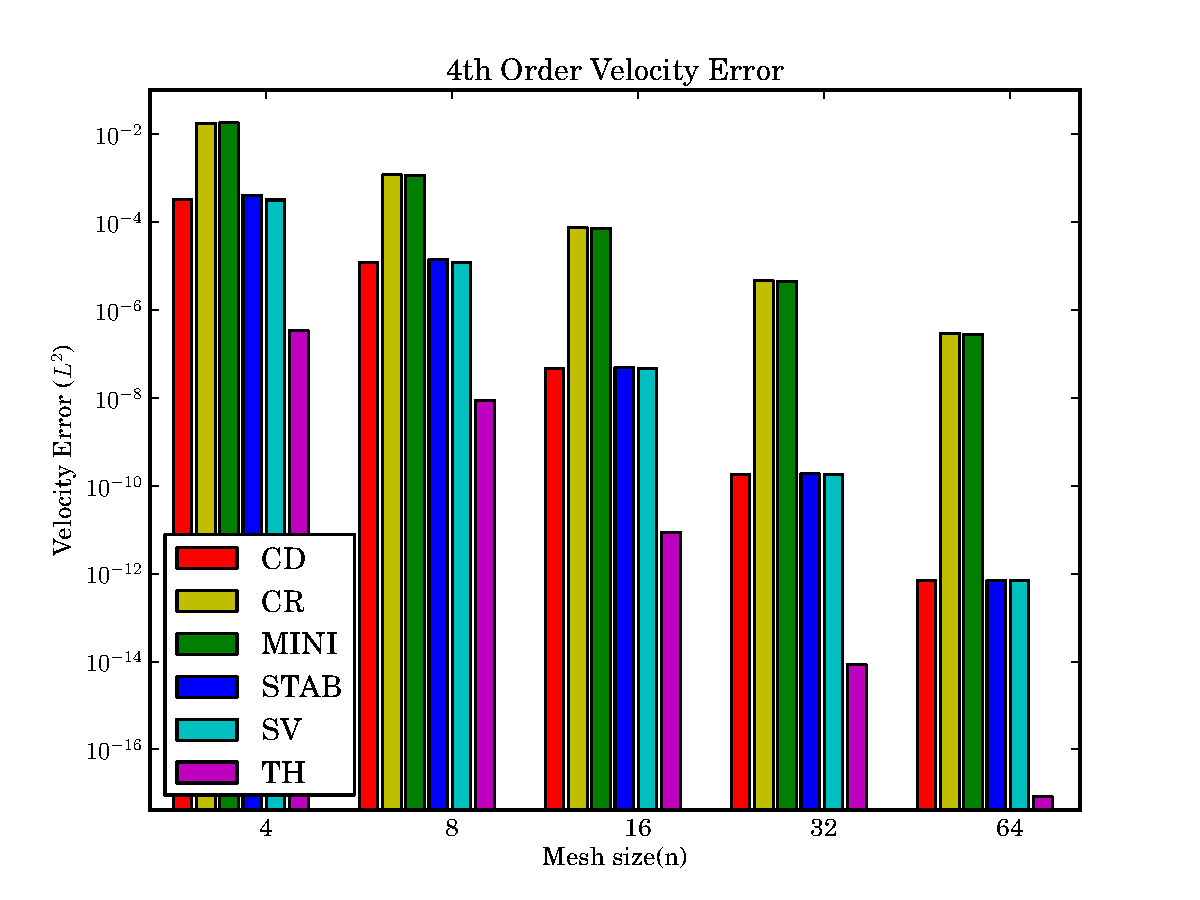
\includegraphics[scale=.65]{chapters/terrel/pdf/vel_4.pdf}
    \label{terrel:fig:4th_Order:vel}
  }
  \subfigure[]{
    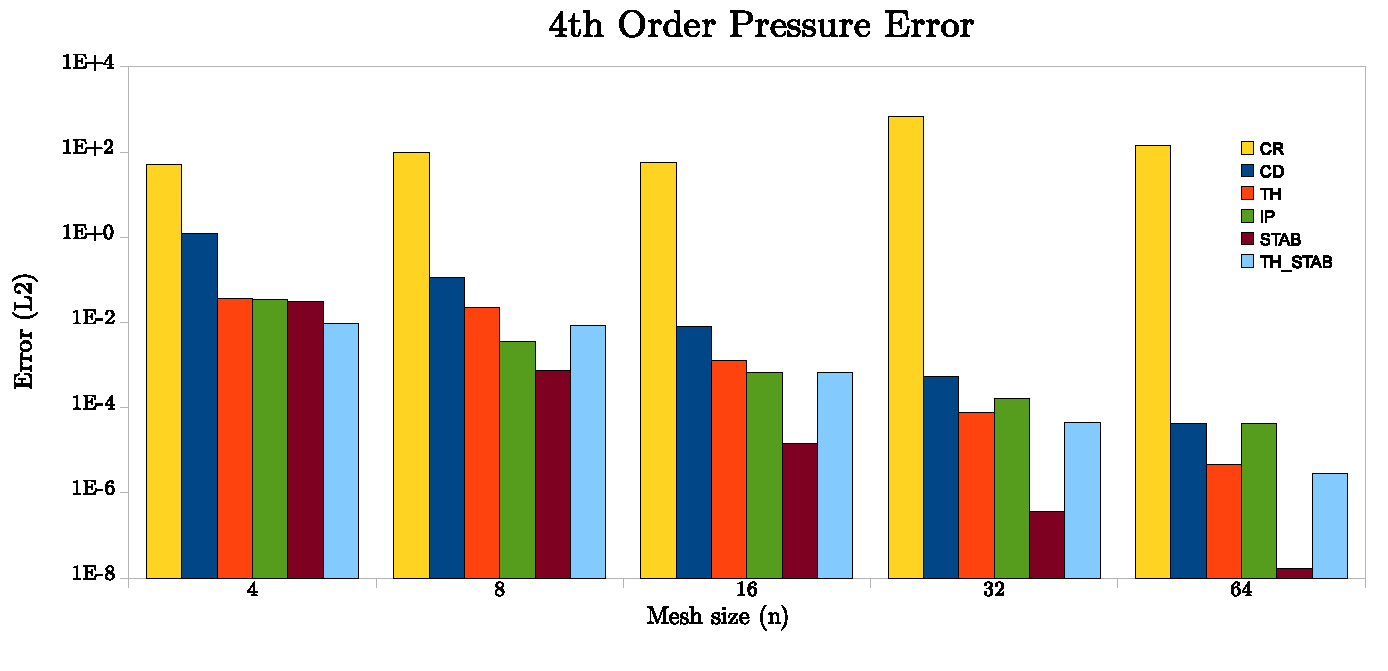
\includegraphics[scale=.65]{chapters/terrel/pdf/press_4.pdf}
    \label{terrel:fig:4th_Order:press}
  }
  \caption{Comparison of 4th Order methods on analytic test case.  Crouzeix-Raviart on a finer mesh
     to have equivalent number of DOFs),TH is Taylor-Hood, IP is Iterated Penalty}
   \label{terrel:fig:4th_Order}
\end{figure}

\begin{figure}
  \subfigure[]{
    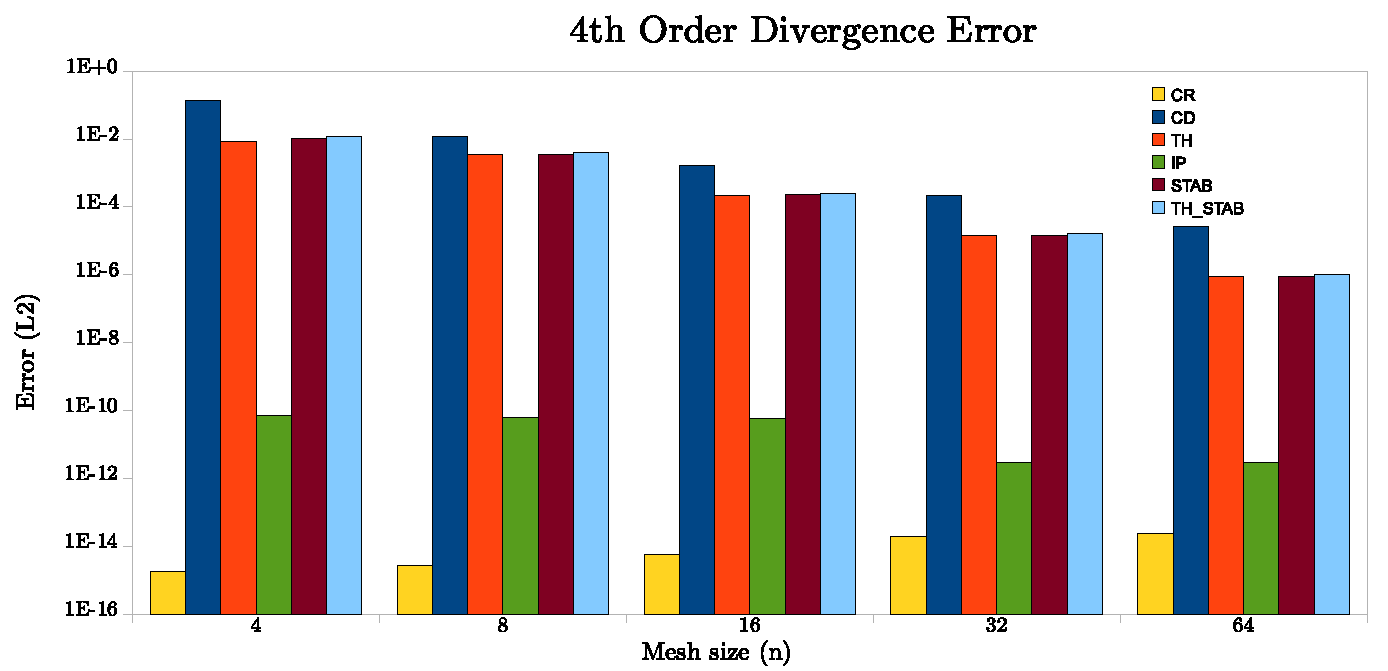
\includegraphics[scale=.65]{chapters/terrel/pdf/div_4.pdf}
    \label{terrel:fig:4th_Order_2:div}
  }
  \subfigure[]{
    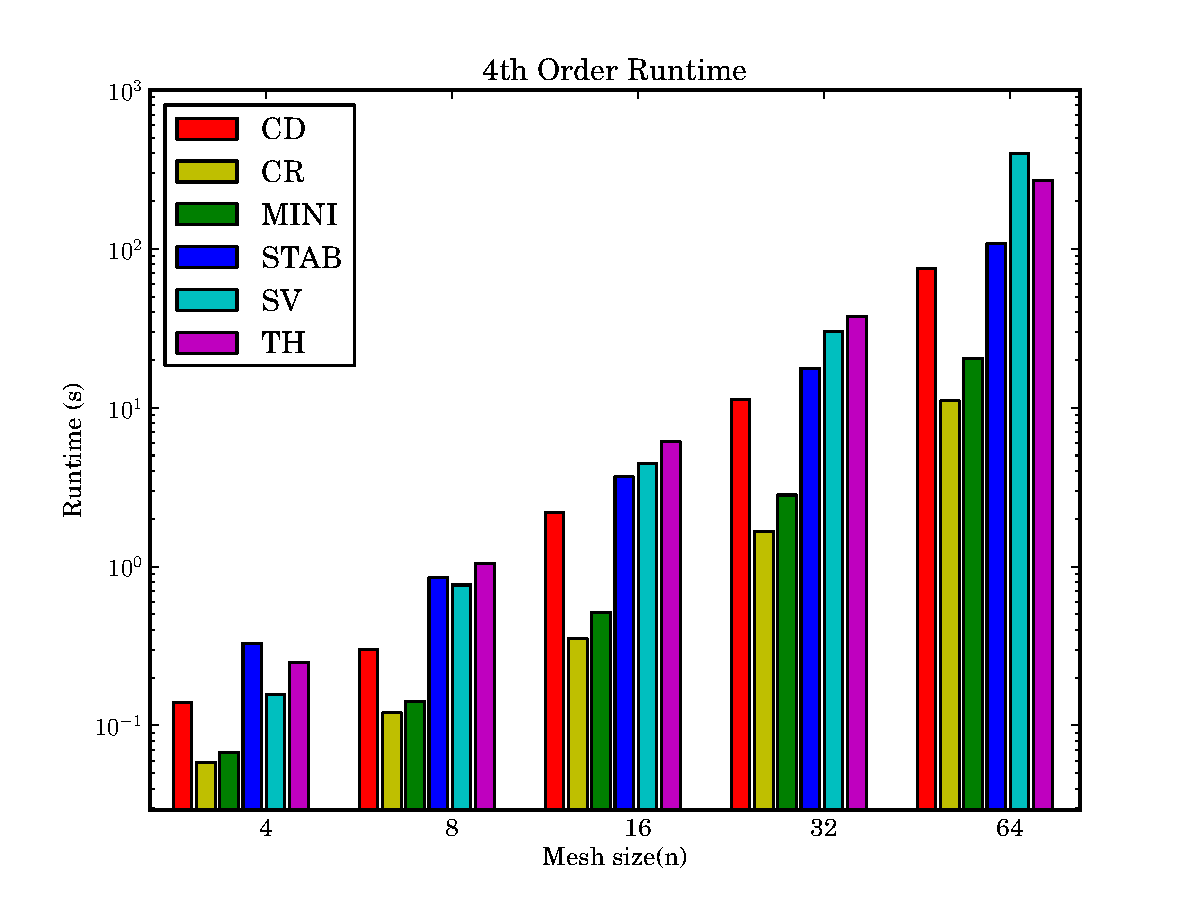
\includegraphics[scale=.65]{chapters/terrel/pdf/run_4.pdf}
    \label{terrel:fig:4th_Order_2:run}
  }
 \caption{Comparison of 4th Order methods on analytic test case, as in Figure~\ref{terrel:fig:4th_Order}}
 \label{terrel:fig:4th_Order_2}
\end{figure}


\begin{figure}
  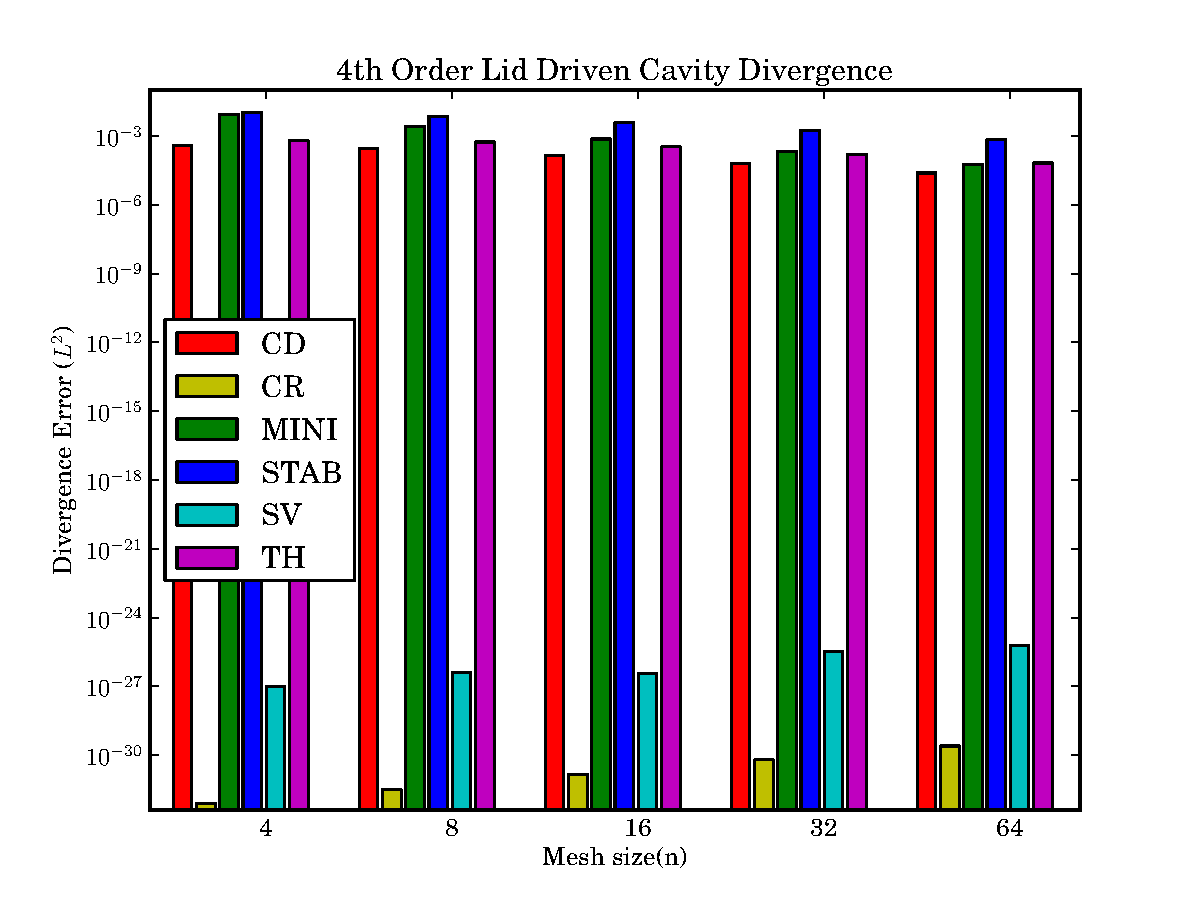
\includegraphics[scale=.65]{chapters/terrel/pdf/div_4_test.pdf}
  \caption{Divergence error comparison of 4th Order methods on lid driven cavity}
  \label{terrel:fig:4th_Order_lid}
\end{figure}


To give a sense of the error,
Figures~\ref{terrel:fig:4th_Order}~and~~\ref{terrel:fig:4th_Order_2} gives a
slice of the data for all fourth order methods with the FEniCS.
Crouzeix-Raviart, with an equivalent number of DOFs, is included in order to
compare with a low order method.  One can see the loss of convergence in
velocity for the CD method due to the low pressure order.  The pressure is
slightly improved with the stabilization parameter for Taylor-Hood but the
ability to use a fourth order representation for the STAB method gives it the
advantage for accuracy.  As theory suggests, the only divergence free methods
are iterated penalty and Crouzeix-Raviart.

Additionally we show the error of the divergence from the lid driven cavity
problem, Figure~\ref{terrel:fig:4th_Order_lid}.  As oppose to the smooth test
case, the divergence error did not decrease as the mesh was refined for
methods which do not conserve the divergence free criteria.  The iterated
penalty parameter had to be increased to 1e8 for the fixed point iteration to
converge.





